% TEX root = lecture/Complex_Analysis 

\begin{center}
    \tikzset{every picture/.style={line width=0.75pt}} %set default line width to 0.75pt        
    
    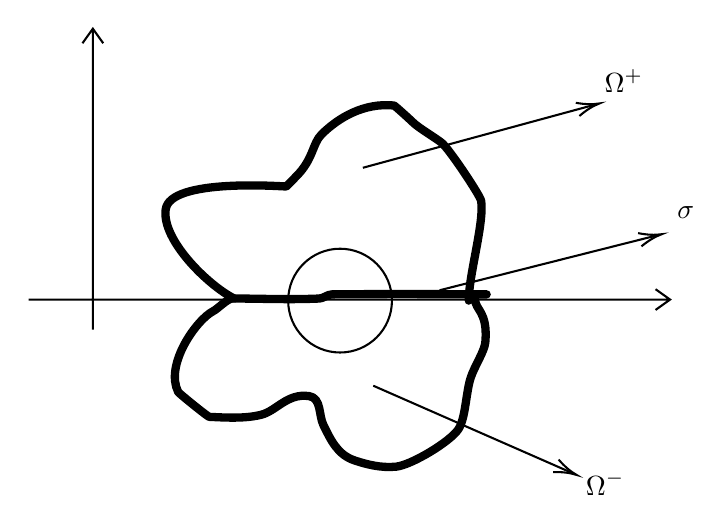
\begin{tikzpicture}[x=0.75pt,y=0.75pt,yscale=-1,xscale=1]
    %uncomment if require: \path (0,392); %set diagram left start at 0, and has height of 392
    
    %Shape: Axis 2D [id:dp13575276746597464] 
    \draw  (175,195.5) -- (484,195.5)(205.9,65) -- (205.9,210) (477,190.5) -- (484,195.5) -- (477,200.5) (200.9,72) -- (205.9,65) -- (210.9,72)  ;
    %Shape: Free Drawing [id:dp14268765045810194] 
    \draw  [line width=3] [line join = round][line cap = round] (274,195) .. controls (261.8,188.9) and (238.88,166.87) .. (241,152) .. controls (243.17,136.83) and (297.23,141.04) .. (299,141) .. controls (299.35,140.99) and (303.48,136.52) .. (304,136) .. controls (312.16,127.84) and (311.69,120.31) .. (316,116) .. controls (324.02,107.98) and (336.42,100.54) .. (351,102) .. controls (351.37,102.04) and (359.04,109.04) .. (360,110) .. controls (362.76,112.76) and (370.64,117.31) .. (374,120) .. controls (377.49,122.8) and (392.64,145.49) .. (393,148) .. controls (394.51,158.55) and (387,183.78) .. (387,196) ;
    %Shape: Free Drawing [id:dp6374095064796427] 
    \draw  [line width=3] [line join = round][line cap = round] (273,195) .. controls (270.83,195) and (265.99,200) .. (264,201) .. controls (256,205) and (240.39,226.79) .. (247,240) .. controls (247.33,240.66) and (261.29,251.97) .. (262,252) .. controls (270.19,252.39) and (279.33,252.92) .. (287,251) .. controls (294.33,249.17) and (299.56,240.51) .. (310,242) .. controls (316.15,242.88) and (314.61,251.22) .. (317,256) .. controls (320.53,263.06) and (323.66,270.22) .. (332,273) .. controls (337.54,274.85) and (344.62,276.74) .. (352,276) .. controls (359.28,275.27) and (377.97,264.05) .. (382,258) .. controls (385.56,252.65) and (385.57,240.3) .. (388,233) .. controls (389.83,227.5) and (394.64,220.34) .. (395,216) .. controls (396.26,200.86) and (390,200.83) .. (390,195) ;
    %Shape: Circle [id:dp9197077331741318] 
    \draw   (300,196) .. controls (300,182.19) and (311.19,171) .. (325,171) .. controls (338.81,171) and (350,182.19) .. (350,196) .. controls (350,209.81) and (338.81,221) .. (325,221) .. controls (311.19,221) and (300,209.81) .. (300,196) -- cycle ;
    %Straight Lines [id:da8903842986356113] 
    \draw    (336,132) -- (448.07,101.52) ;
    \draw [shift={(450,101)}, rotate = 164.79] [color={rgb, 255:red, 0; green, 0; blue, 0 }  ][line width=0.75]    (10.93,-3.29) .. controls (6.95,-1.4) and (3.31,-0.3) .. (0,0) .. controls (3.31,0.3) and (6.95,1.4) .. (10.93,3.29)   ;
    %Straight Lines [id:da4166743347978691] 
    \draw    (341,237) -- (437.17,279.2) ;
    \draw [shift={(439,280)}, rotate = 203.69] [color={rgb, 255:red, 0; green, 0; blue, 0 }  ][line width=0.75]    (10.93,-3.29) .. controls (6.95,-1.4) and (3.31,-0.3) .. (0,0) .. controls (3.31,0.3) and (6.95,1.4) .. (10.93,3.29)   ;
    %Shape: Free Drawing [id:dp9885674880852715] 
    \draw  [line width=3] [line join = round][line cap = round] (274,195) .. controls (287.22,195) and (299.93,195.63) .. (315,195) .. controls (317.11,194.91) and (318.89,193.03) .. (321,193) .. controls (344.33,192.68) and (414.33,193) .. (391,193) ;
    %Straight Lines [id:da3473062677735872] 
    \draw    (373,191) -- (478.06,164.49) ;
    \draw [shift={(480,164)}, rotate = 165.84] [color={rgb, 255:red, 0; green, 0; blue, 0 }  ][line width=0.75]    (10.93,-3.29) .. controls (6.95,-1.4) and (3.31,-0.3) .. (0,0) .. controls (3.31,0.3) and (6.95,1.4) .. (10.93,3.29)   ;
    
    % Text Node
    \draw (451,83) node [anchor=north west][inner sep=0.75pt]   [align=left] {$\displaystyle \Omega ^{+}$};
    % Text Node
    \draw (442,277) node [anchor=north west][inner sep=0.75pt]   [align=left] {$\displaystyle \Omega ^{-}$};
    % Text Node
    \draw (486,149) node [anchor=north west][inner sep=0.75pt]   [align=left] {$\displaystyle \sigma $};
    
    
    \end{tikzpicture}
\end{center}
\begin{proof}
    
    $ h(z)=\begin{cases}
        v(z),&z\in \Omega^+\\
        0,&z\in\sigma\\
        v(\bar{z}),&z\in\Omega^-
    \end{cases} $.

    We need to prove that  $ h $ is harmonic in  $ \Omega $. It suffices to prove  $ h  $ is harmonic on  $ \sigma $. Choose  $ \delta  $ small \st  $ \overline{B(x,\delta)}\subset \Omega $. Let  $ P_h  $ be the Poisson integral  w.r.t.  $ \partial B(x_0,\delta) $ with the boundary values  $ h  $.

    Schwarz' theorem \ref{thm:5.6.4:Schwarz's theorem} implies  $ P_h $ is harmonic in  $ \overline{B(x,\delta)} $ and continuous on  $ \overline{B(x_0,\delta)} $. It follows that,
    
    (1) $ v-P_h $ is harmonic in the upper half disk  $ B(x_0,\delta)\cap\{z\in\Cbb:\Imag z>0\} $. 

    (2) $ v-P_h=0 $ on  $ \partial B(x,\delta)\cap\{z\in\Cbb:\Imag z \geq 0\} $.  

    $ \forall x\in B(x_0,\delta)\cap \sigma $, apply Poisson formula \ref{eq:5.6.3:Poisson's formula}
    \begin{equation}
        P_h(x)=\frac{1}{2\pi}\int_0^{2\pi}\dps\frac{\delta^2-|x|^2}{|\delta e^{i\theta}-x|^2}h(\delta e^{i\theta})\dd\theta=0
    \end{equation} 
    by symmetry.

    Apply the maximum and  minimum principle \ref{cor:5.6.2:u1=u2 iff u1=u2 on the boundary} to  $ h-P_h $, we get  $ h=P_h $ in  $ B(x,\delta)\cap\{z\in \Cbb:\Imag z \geq 0\} $.
    
    The same argument works for the lower half disk.

    So  $ h=P_h  $ in  $ B(x_0,\delta) $ $ \Rightarrow  $  $ h  $ is harmonic at  $ x_0 $.
    
    For the second part of the theorem, it is enough to prove  $ \tilde{f}(z)=\begin{cases}
        f(z),&z\in\Omega^+\\
        \overline{f(\bar{z})},&z\in\Omega^-
    \end{cases} $ 
    is analytic on  $ \sigma $.
    
    For  $ \forall x_0\in\sigma $, let  $ B(x_0,\delta) $ be as before. We already proved  $ v  $ can be extended to a harmonic function in  $ B(x_0,\delta) $.  $ v  $ has a conjugate function  $ -u_0 $ iin the same disk. We may normalize  $ u_0  $ \st  $ u_0=\Real f(z) $  in  $ B(x_0,\delta\cap\{z\in\Cbb,\Imag z>0\}) $. Define  $ g(z):=u_0(z)-u_0(\bar{z}) $.
    
    Then  $ g(x)=0 $ for  $ x\in B(x_0,\delta)\cap \sigma $ $ \Rightarrow  $ 
    \begin{align*}
        \frac{\partial g}{\partial x}(z)=0,\,\forall z\in B(x_0,\delta)\cap\sigma\\
        \frac{\partial g}{\partial y}(x)=2\frac{\partial u_0}{\partial y}(z)=-2\frac{\partial v}{\partial x}(z)=0
    \end{align*}  

    So the analytic function  $ \dps\frac{\partial g}{\partial x}-i\frac{\partial g}{\partial y}\equiv 0 $ on   $ B(x,\delta)\cap \sigma $.(It is analytic because of \eqref{eq:5.6.1:harmonic function induces an anlytic function}) Then  $ \dps\frac{\partial g}{\partial x}-i\frac{\partial g}{\partial y}\equiv 0 $  in  $ B(x_0,\delta) $ $ \Rightarrow  $   $ g\equiv 0 $.
    
    So  $ u_0(z)=u_0(\bar{z}) $,  $ \forall z\in B(x_0,\delta) $  $ \Rightarrow  $  $ f(z)=u_0(z)+i v(z) $ is analytic in  $ B(x_0,\delta) $ and  $ f(z)=\overline{f(\bar{z})} $ for  $ \forall z\in B(x_0,\delta) $.



\end{proof}

\begin{remark}
    The reflection principle can be applied to any circles with symmetric points by using M{\"o}bius transformation. However, the condition of $ f(\Rbb)\subset \Rbb $ (\ie  $ v(\Rbb)=0) $ transforms to  $ f(C)\subset C $. 
\end{remark}

\section{Series and Product Representations}
\subsection{Power Series Expansions}
\subsubsection{Weierstrass's Theorem}
\begin{theorem}[Weierstrass's Theorem]\label{thm:5.1.1:Weierstrass's Theorem}
    Suppose  $ f_n  $ is analytic in the region  $ \Omega_n  $ for each  $ n\in \Nbb  $, and  $ \Omega_1\subset \Omega_2\subset\cdots\subset\Omega_n\subset\cdots $ and  $ \dps\bigcup_{n\in \Nbb}\Omega_n=\Omega $. If  $ f_n  $ converges to  $ f  $ in  $ \Omega  $, uniformly on every compact subset of  $ \Omega  $, then  $ f $ is analytic in  $ \Omega  $. 

    Moreover,  $ f_n' $ converges uniformly to  $ f' $ on every compact subset of  $ \Omega $.  
\end{theorem}
\begin{proof}
    $ \forall  $ compact subset  $ K\subset \Omega  $,  $ K\subset\dps \bigcup\limits_{n=1}^\infty \Omega_n$ $ \Rightarrow $   $ \exists N\in \Nbb $ such that  $ K\subset \dps\bigcup_{n=1}^{N}\Omega_n $.

    $ \forall z_0\in \Omega $,  $ \exists   R>0 $ \st  $ \overline{B(z_0,R)}\subset \Omega $. Choose  $ N\in \Nbb $ \st  $ \overline{B(z_0,R)}\subset \Omega_n $ for  $ \forall n \geq N $.
    
    Cauchy's integral formula \ref{General form of Cauchy's theorem} implies 
    \begin{equation}
        f_n(z)=\frac{1}{2\pi i}\int_{\partial B(z_0,R)}\frac{f_n(\zeta)}{\zeta-z}\dd\zeta,\,\forall z\in B(z_0,R)
    \end{equation}

    $ f_n\rightrightarrows f  $ uniformly on  $ \overline{B(z_0,R)} $  $ \Rightarrow  $ 
    \begin{equation}
        f(z)=\frac{1}{2\pi i}\int_{\partial B(z_0,R)}\frac{f(\zeta)}{\zeta-z}\dd\zeta
    \end{equation} 
    Then  $ f  $ is  analytic in  $ B(z_0,R)$ by lemma \ref{sec5.2.3:Lemma of Analytic Properties of integral function}.

    \begin{equation}
        \begin{cases}
            f_n'(z)=\dps\frac{1}{2\pi i}\int_{\partial B(z_0,R)}\frac{f_n(\zeta)}{(\zeta-z)^2}\dd\zeta&\forall z\in B(z_0,R)\\
            f'(z)=\dps\frac{1}{2\pi i}\int_{\partial B(z_0,R)}\frac{f(\zeta)}{(\zeta-z)^2}\dd\zeta&\forall z\in B(z_0,R)
        \end{cases}
    \end{equation}
    Then  $ |f_n'(z)-f'(z)| \leq\dps \frac{1}{2\pi}\int_{\partial B(z_0,R)}\dps\frac{|f_n(\zeta)-f(\zeta)|}{|\zeta-z|^2}|\dd\zeta| $. Therefore,  $ f_n'  $ uniformly converges to  $ f' $ in  $ B(z_0,\rho ) $ for  $ 0<\rho<R$.    

    Since any compact subset of  $ \Omega  $ can be covered by a finite number of such closed disks,  $ f_n\rightrightarrows f$ uniformly on every compact subset of  $ \Omega  $.
\end{proof}
\begin{corollary}\label{cor:5.1.1:Corollary of Weierstrass's Theorem}
    If  $ f_n  $ is analytic in a region  $ \Omega  $ for  $ n\in \Nbb  $, and  $ \dps\sum_{j=1}^n f_j\rightrightarrows f $ on every compact subset of  $ \Omega $, then  $ f  $ is analytic  in  $ \Omega  $ and $ f'(z)=\dps\sum_{j=1}^\infty f_j'(z),\,\forall z\in \Omega $ uniformly on every compact subset of  $ \Omega $.
\end{corollary}
\begin{theorem}[Hurwitz's Theorem]\label{thm:5.1.1:Hurwitz's Theorem}
    If the functions  $ f_n  $ are analytic and nowhere zero in a region  $ \Omega  $, and if  $ f_n\rightrightarrows f $ on every compact subset of  $ \Omega $, then  $ f  $ is either identically zero or never equal to  $ 0  $ in  $ \Omega $.    
\end{theorem}
\begin{proof}
    Suppose  $  f \not\equiv 0 $. The zeros of  $ f  $ are isolated.

     $ \forall z_0\in \Omega  $,  $ \exists \delta>0  $ \st  $ f(z)\neq 0 $,  $ \forall z\in B(z_0,\delta)\setminus \{z_0\}\subset\Omega $.
     
     Then  $ |f|  $ has a positive minimum on  $ \partial B(z_0,\delta) $. Thus, $ \dps\frac{1}{f_n}\rightrightarrows \frac{1}{f} $ on  $ \partial B(z_0,\delta) $.
     
    Combined with $ f_n'\rightrightarrows f' $ on  $ \partial B(z_0,\delta) $  $ \Rightarrow $
    \begin{equation}
        \lim_{n\to\infty}\frac{1}{2\pi i}\int_{\partial B(z_0,\delta)}\frac{f_n'(z)}{f_n(z)}\dd z=\frac{1}{2\pi i}\int_{\partial B(z_0,\delta)}\frac{f'(z)}{f(z)}\dd z
    \end{equation}  
    By argument principle \ref{The Argument Principle}, this equation equals to  $ 0 $. So  $ f  $ has no zeros on  $ \partial B(z_0,\delta) $, so is on  $ \Omega $. 
\end{proof}